


 Consider a standard number line with points located at $x, x^{2}, x^{3}$ as shown below.
\begin{center}
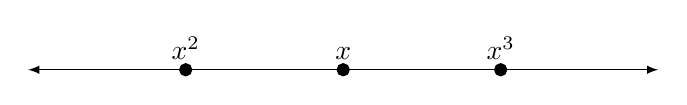
\begin{tikzpicture}
\draw[>=latex,<->](0,0)--(8,0);
    \draw[thick, fill=black] (2,0) circle (.07cm) node[above]{$x^{2}$};
    \draw[thick, fill=black] (4,0) circle (.07cm) node[above]{$x$};
    
      \draw[thick, fill=black] (6,0) circle (.07cm)  node[above]{$x^{3}$};
\end{tikzpicture}
\end{center}
Which of the following describe all possible $x$?


\ifsat
	\begin{enumerate}[label=\Alph*)]
		\item    $0<x<1$
		\item $-1<x<0$
		\item $1<x$
		\item  No such $x$ exists. %
	\end{enumerate}
\else
\fi

\ifacteven
	\begin{enumerate}[label=\textbf{\Alph*.},itemsep=\fill,align=left]
		\setcounter{enumii}{5}
		\item    $0<x<1$
		\item $-2<x$ 
		\item $-1<x<0$
		\addtocounter{enumii}{1}
		\item $1<x$
		\item  No such $x$ exists. %
	\end{enumerate}
\else
\fi

\ifactodd
	\begin{enumerate}[label=\textbf{\Alph*.},itemsep=\fill,align=left]
		\item    $0<x<1$
		\item $-2<x$ 
		\item $-1<x<0$
		\item $1<x$
		\item  No such $x$ exists. %
	\end{enumerate}
\else
\fi

\ifgridin
  No such $x$ exists. %

\else
\fi

